% Figure 2: GNN track-to-vertex association. Standalone TikZ; compiled by diagrams.py.
% Content follows the technical note, Sections 7.2-7.3 (fig:gnn_graph) and
% src/gnn/models/ttva_gat.py (TTVAGATModel).
\documentclass[tikz,border=4pt]{standalone}
\usepackage[T1]{fontenc}
\usepackage{helvet}
\renewcommand{\familydefault}{\sfdefault}
\usepackage{amsmath}
\usepackage{sansmath}
\sansmath
\usetikzlibrary{arrows.meta,positioning,calc,decorations.pathreplacing,fit,backgrounds}
\definecolor{nn}{HTML}{0072B2}
\definecolor{vx}{HTML}{D55E00}
\definecolor{io}{gray}{0.55}
\begin{document}
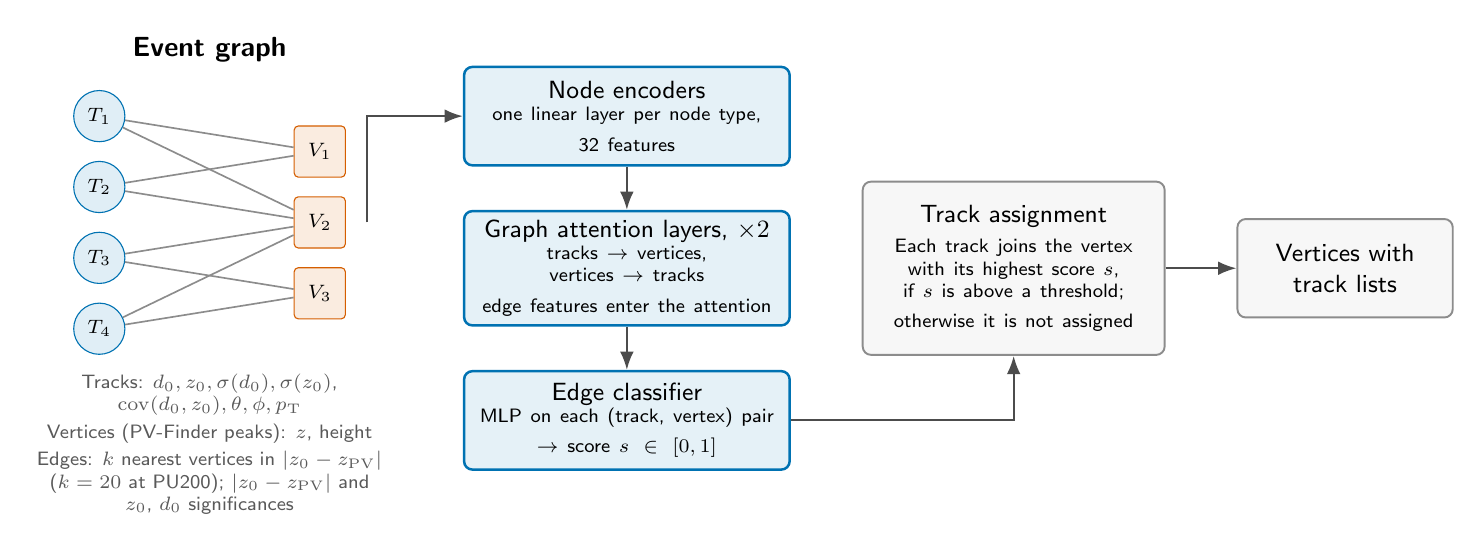
\begin{tikzpicture}[
  >=Latex, font=\small,
  trk/.style={circle, draw=nn, fill=nn!12, minimum size=6.5mm, inner sep=0pt, font=\scriptsize},
  vtx/.style={rectangle, rounded corners=1.5pt, draw=vx, fill=vx!12, minimum size=6.5mm,
              inner sep=0pt, font=\scriptsize},
  box/.style={draw=io, rounded corners=3pt, fill=black!3, align=center,
              text width=3.1cm, minimum height=1.25cm, line width=0.7pt},
  net/.style={draw=nn, rounded corners=3pt, fill=nn!10, align=center,
              text width=3.9cm, minimum height=1.25cm, line width=0.9pt},
  arr/.style={->, line width=0.8pt, draw=black!70},
  dim/.style={font=\scriptsize, text=black!65, align=center},
]
  % ---- (a) Graph ------------------------------------------------------------
  \node[font=\bfseries] at (1.4,3.15) {Event graph};
  \node[trk] (t1) at (0,2.3) {$T_1$};
  \node[trk] (t2) at (0,1.4) {$T_2$};
  \node[trk] (t3) at (0,0.5) {$T_3$};
  \node[trk] (t4) at (0,-0.4) {$T_4$};
  \node[vtx] (v1) at (2.8,1.85) {$V_1$};
  \node[vtx] (v2) at (2.8,0.95) {$V_2$};
  \node[vtx] (v3) at (2.8,0.05) {$V_3$};
  \foreach \t/\v in {t1/v1, t1/v2, t2/v1, t2/v2, t3/v2, t3/v3, t4/v2, t4/v3}
    \draw[black!45, line width=0.6pt] (\t) -- (\v);
  \node[dim, anchor=north] at (1.4,-0.85)
    {Tracks: $d_0, z_0, \sigma(d_0), \sigma(z_0)$,\\$\mathrm{cov}(d_0,z_0), \theta, \phi, p_{\mathrm{T}}$\\[2pt]
     Vertices (PV-Finder peaks): $z$, height\\[2pt]
     Edges: $k$ nearest vertices in $|z_0-z_{\mathrm{PV}}|$\\
     ($k=20$ at PU200); $|z_0-z_{\mathrm{PV}}|$ and\\
     $z_0$, $d_0$ significances};

  % ---- (b) Network ----------------------------------------------------------
  \node[net] (enc) at (6.7,2.3)
    {Node encoders\\\scriptsize one linear layer per node type,\\\scriptsize 32 features};
  \node[net, below=0.55cm of enc] (gat)
    {Graph attention layers, $\times 2$\\\scriptsize tracks $\to$ vertices, vertices $\to$ tracks\\\scriptsize edge features enter the attention};
  \node[net, below=0.55cm of gat] (mlp)
    {Edge classifier\\\scriptsize MLP on each (track, vertex) pair\\\scriptsize $\to$ score $s\in[0,1]$};
  \draw[arr] (enc) -- (gat);
  \draw[arr] (gat) -- (mlp);
  \draw[arr] (3.4,0.95) |- (enc.west);

  % ---- (c) Assignment -------------------------------------------------------
  \node[box, right=0.9cm of gat, text width=3.6cm, minimum height=2.2cm] (assign)
    {Track assignment\\[3pt]
     \scriptsize Each track joins the vertex\\\scriptsize with its highest score $s$,\\\scriptsize if $s$ is above a threshold;\\\scriptsize otherwise it is not assigned};
  \draw[arr] (mlp.east) -| (assign.south);

  % Output.
  \node[box, right=0.9cm of assign, text width=2.5cm] (out)
    {Vertices with\\track lists};
  \draw[arr] (assign) -- (out);
\end{tikzpicture}
\end{document}
